\section{MFCC Computation}

\begin{frame}[fragile,allowframebreaks]{MFCC Computation}
    \begin{itemize}
    \item MFCCs are widely used in speech and audio processing.
    \item They capture the timbral texture of audio signals.
    \item Typically, only the first 13 coefficients are used for feature extraction.
\end{itemize}
\framebreak
\begin{figure}
    \centering
    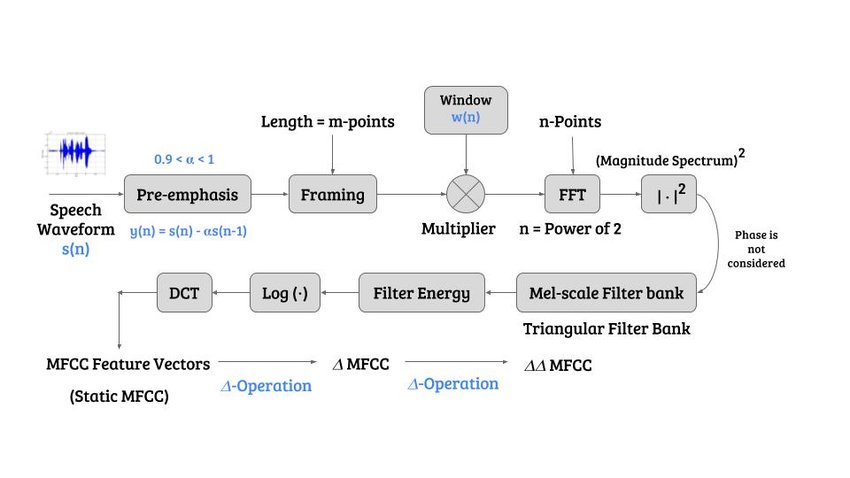
\includegraphics[width=1.08\textwidth,height=0.8\textheight,keepaspectratio]{images/audio-nlp/mfcc.png}
    \caption*{A block diagram for MFCC computation: From audio signal to MFCC features.}
\end{figure}
\framebreak
\textbf{Pipeline:}
\begin{enumerate}
    \item Compute log-Mel spectrogram
    \item Apply Discrete Cosine Transform (DCT)
    \item Keep first 13 coefficients (MFCCs)
\end{enumerate}

\textbf{MFCC Equation:}
\begin{equation}
    c_k = \sum_{n=1}^{N} \log(E_n) \cos\left[ \frac{\pi k}{N} \left( n - \frac{1}{2} \right) \right]
\end{equation}
where:
\begin{itemize}
    \item $c_k$ is the $k$-th MFCC coefficient
    \item $E_n$ is the energy in the $n$-th Mel filter
    \item $N$ is the total number of Mel filters
\end{itemize}
\end{frame}